%%%%%%%%%%%%%%%%%%%%%%%%%%%%%%%%%%%%%%%
% Wenneker Resume/CV
% LaTeX Template
% Version 1.1 (19/6/2016)
%
% This template has been downloaded from:
% http://www.LaTeXTemplates.com
%
% Original author:
% Frits Wenneker (http://www.howtotex.com) with extensive modifications by 
% Vel (vel@LaTeXTemplates.com)
%
% License:
% CC BY-NC-SA 3.0 (http://creativecommons.org/licenses/by-nc-sa/3.0/
%
%%%%%%%%%%%%%%%%%%%%%%%%%%%%%%%%%%%%%%

%----------------------------------------------------------------------------------------
%	PACKAGES AND OTHER DOCUMENT CONFIGURATIONS
%----------------------------------------------------------------------------------------

\documentclass[a4paper,12pt]{memoir} % Font and paper size
\usepackage{multicol}
%%%%%%%%%%%%%%%%%%%%%%%%%%%%%%%%%%%%%%%%%
% Wenneker Resume/CV
% Structure Specification File
% Version 1.1 (19/6/2016)
%
% This file has been downloaded from:
% http://www.LaTeXTemplates.com
%
% Original author:
% Frits Wenneker (http://www.howtotex.com) with extensive modifications by 
% Vel (vel@latextemplates.com)
%
% License:
% CC BY-NC-SA 3.0 (http://creativecommons.org/licenses/by-nc-sa/3.0/)
%
%%%%%%%%%%%%%%%%%%%%%%%%%%%%%%%%%%%%%%%%%

%----------------------------------------------------------------------------------------
%	PACKAGES AND OTHER DOCUMENT CONFIGURATIONS
%----------------------------------------------------------------------------------------

\usepackage{XCharter} % Use the Bitstream Charter font
\usepackage[utf8]{inputenc} % Required for inputting international characters
\usepackage[T1]{fontenc} % Output font encoding for international characters

\usepackage[top=1cm,left=1cm,right=1cm,bottom=1cm]{geometry} % Modify margins

\usepackage{graphicx} % Required for figures

\usepackage{flowfram} % Required for the multi-column layout

\usepackage{url} % URLs

\usepackage[usenames,dvipsnames]{xcolor} % Required for custom colours

\usepackage{tikz} % Required for the horizontal rule

\usepackage[danish]{babel}

\usepackage{enumitem} % Required for modifying lists
\setlist{noitemsep,nolistsep} % Remove spacing within and around lists

\setlength{\columnsep}{\baselineskip} % Set the spacing between columns

% Define the left frame (sidebar)
\newflowframe{0.2\textwidth}{\textheight}{0pt}{0pt}[left]
\newlength{\LeftMainSep}
\setlength{\LeftMainSep}{0.2\textwidth}
\addtolength{\LeftMainSep}{1\columnsep}
 
% Small static frame for the vertical line
\newstaticframe{1.5pt}{\textheight}{\LeftMainSep}{0pt}
 
% Content of the static frame with the vertical line
\begin{staticcontents}{1}
\hfill
\tikz{\draw[loosely dotted,color=RoyalBlue,line width=1.5pt,yshift=0](0,0) -- (0,\textheight);}
\hfill\mbox{}
\end{staticcontents}
 
% Define the right frame (main body)
\addtolength{\LeftMainSep}{1.5pt}
\addtolength{\LeftMainSep}{1\columnsep}
\newflowframe{0.7\textwidth}{\textheight}{\LeftMainSep}{0pt}[main01]

\pagestyle{empty} % Disable all page numbering

\setlength{\parindent}{0pt} % Stop paragraph indentation

%----------------------------------------------------------------------------------------
%	NEW COMMANDS
%----------------------------------------------------------------------------------------

\newcommand{\userinformation}[1]{\renewcommand{\userinformation}{#1}} % Define a new command for the CV user's information that goes into the left column

\newcommand{\cvheading}[1]{{\Huge\bfseries\color{RoyalBlue} #1} \par\vspace{.6\baselineskip}} % New command for the CV heading
\newcommand{\cvsubheading}[1]{{\Large\bfseries #1} \bigbreak} % New command for the CV subheading

\newcommand{\Sep}{\vspace{1em}} % New command for the spacing between headings
\newcommand{\SmallSep}{\vspace{0.5em}} % New command for the spacing within headings

\newcommand{\aboutme}[2]{ % New command for the about me section
\textbf{\color{RoyalBlue} #1}~~#2\par\Sep
}
	
\newcommand{\CVSection}[1]{ % New command for the headings within sections
{\Large\textbf{#1}}\par
\SmallSep % Used for spacing
}

\newcommand{\CVItem}[2]{ % New command for the item descriptions
\textbf{\color{RoyalBlue} #1}\par
#2
\SmallSep % Used for spacing
}

\newcommand{\bluebullet}{\textcolor{RoyalBlue}{$\circ$}~~} % New command for the blue bullets
 % Include the file specifying document layout and packages

%----------------------------------------------------------------------------------------
%	NAME AND CONTACT INFORMATION 
%----------------------------------------------------------------------------------------

\userinformation{ % Set the content that goes into the sidebar of each page
\begin{flushright}
% Comment out this figure block if you don't want a photo
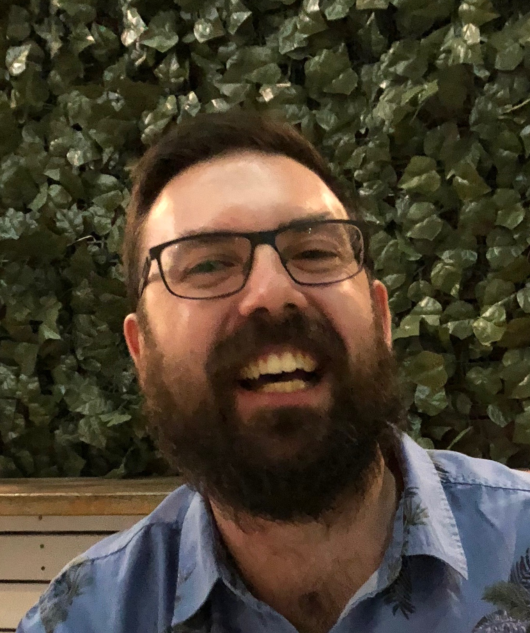
\includegraphics[width=0.6\columnwidth]{nathan.png}\\[\baselineskip] % Your photo
\small % Smaller font size
Nathan Hugh Barr \\ % Your name
\Sep
\url{nathanhbarr@gmail.com} \\ % Your email address
\Sep

tlf: +45 61 73 55 92 \\ % Your phone number
\Sep % Some whitespace
\textbf{Address} \\
Østerbrogade 202, 4.tv \\ % Address 1
2100 København Ø \\ % Address 2
% \\ % Address 3
\Sep
\url{www.linkedin.com/in/nathanhbarr/} \\ % Your URL
\vfill % Whitespace under this block to push it up under the photo
\end{flushright}
}

%----------------------------------------------------------------------------------------

\begin{document}

\userinformation % Print your information in the left column

\framebreak % End of the first column

%----------------------------------------------------------------------------------------
%	HEADING
%----------------------------------------------------------------------------------------

\cvheading{Nathan Hugh Barr} % Large heading - your name

\cvsubheading{} % Subheading - your occupation/specialization

%----------------------------------------------------------------------------------------
%	ABOUT ME
%----------------------------------------------------------------------------------------

%As a Cand.Scient in Physics and Mathematics, I consider myself as a generalist. Throughout my coursework and projects, I have relied on my ability to quickly immerse myself in topics and research areas. I have had to use concepts and techniques found in other scientific areas to complete my projects. A core ability that I have received during my tertiary education is the ability to be a problem-solver, being able pursue solutions in any area of science. My past jobs have been more focused on academia and teaching, but presently I am looking for new challenges in research and analytics. I am not shy when receiving constructive criticism and I am able to incorporate them immediately. I work well in a team environment. My Cand.Scient degree in Physics and mathematics has given me .

%\aboutme{Profile}{I have performed data analysis throughout my tertiary education on many types of data sets, ranging from small to large, complete and incomplete. These data sets have not only encompassed my field of study, physics and mathematics but also biology and chemistry. I can contribute my past experiences working with these different types of data sets to this position. I can perform both mathematical and numerical analysis on data sets and on mathematical models. I am versed in data analysis using python and matlab and i am quick to pickup any programming languages this position requires. I have experience in building mathematical models from the ground up using both text book theory and research from published articles. I have a wealth of experience working in project groups which i can contribute to this position through my ease of working in a team environment and my ability to immerse myself quickly in the project. }

%{I have extensive experience with the analysis of many types of data sets, ranging from small to large, complete and incomplete. I also have experience in building mathematical models from the ground up using both text book theory and research from published articles. This skill set, I believe, can be useful in this position in the development of new predictive models and reporting the results and analysis quickly.}


\aboutme{Professional Profile:}{Jeg er en nyuddannet Cand.Scient i Fysik og Matematik som har erfaring indenfor programmering og kan drive et projekt selvstændig. Gennem min uddannelse har jeg programmeret i Matlab og Octave, som jeg har brugt til at simulere og modellere fysiske fænomener, som f.eks. hvor hurtigt oxygen diffunderer igennem hvidvin og oxiderer med ethanol. I min fritid efter uddannelsen, læser jeg selv op på, hvordan man programmerer i Python, hvordan man bruger SQL-sprog og databaser, og hvordan man kan implementere machine learning algoritmer ved at bruge pakken scikit-learn. Min uddannelse på RUC har bestået af $50\%$ kurser og $50\%$ projekter. Vi er blevet uddannet i at drive tværfaglige projekter, der undersøger en problemstilling og bidrager til videnskaben. Jeg har erfaring med projektstyring og -ledelse, og jeg kan overholde en deadline. Mine uddannelse har givet mig en analytisk og struktureret tilgang til både at researche og løse problemer. Mit modersmål er engelsk, så jeg kan kommunikere både på dansk og engelsk. Jeg er en optimistisk og rar person, som leder efter udfordringer og ansvar.
}

%----------------------------------------------------------------------------------------
%	EDUCATION
%----------------------------------------------------------------------------------------

\CVSection{Education}


%------------------------------------------------

\CVItem{2016 - 2019, Roskilde University}{Master of Science in Physics and Mathematics\\
\small Master Thesis: 
\begin{itemize}
\item Title: \textit{Optimising the thickness determination of homopolymers and diblock copolymers using optical spectral reflectance during solvent vapour annealing.}
\item Collecting, analysing and visualising data.
\item Programming models and fitting routines. 
\item Grade: 10 
\end{itemize}}

%------------------------------------------------

\CVItem{2013 - 2016, Roskilde Universitet}{Bachelor of Natural Science in Physics and Mathematics\\
\small Bachelor project: 
\begin{itemize}
\item Title: \textit{Mathematical competencies gained in Danish High School Education from 1958 to the present - using integrals as a case study.} 
\item Grade: 10
\end{itemize}
}

%------------------------------------------------

\CVItem{Relevant Courses}{}
\begin{itemize}
\item Calculus
\item Mathematical Modelling
\item Probability and Statistics
\item Statistical Mechanics
\end{itemize}


%------------------------------------------------

\Sep % Extra whitespace after the end of a major section

%----------------------------------------------------------------------------------------
%	EXPERIENCE
%----------------------------------------------------------------------------------------

\CVSection{Experience and Volunteering}

%------------------------------------------------

\CVItem{September 2016 and September 2017, \textit{Teachers Assistant-RUC}, Data processing and Statistics.}{}
\begin{itemize}
	\item Teaching - basic programming, scripting and functions.
	\item Teaching - Introduction statistics in natural science.	
\end{itemize}

%------------------------------------------------

\CVItem{January 2015 - December 2018, \textit{Private tutor}, My academy.}{}

%------------------------------------------------

\CVItem{October 2015 - December 2018, \textit{Science Show Representative}, Roskilde University.}{}

%------------------------------------------------

\CVItem{June 2017 - June 2019, \textit{Co-creator at Roskilde Festival}, Volunteering.}{}


\Sep % Extra whitespace after the end of a major section
%----------------------------------------------------------------------------------------
%	SKILLS
%----------------------------------------------------------------------------------------

\clearpage % Start a new page

\userinformation % Print your information in the left column

\framebreak % End of the first column


\CVSection{Technical skills}

%------------------------------------------------

\CVItem{Programming and systems}
{\begin{tabular}{p{0.2\textwidth} p{0.2\textwidth} p{0.2\textwidth} }
		\bluebullet GNU Octave &  \bluebullet MatLab & \bluebullet Python\\
\end{tabular}}


%------------------------------------------------

\CVItem{Computer Software}
{\begin{tabular}{p{0.2\textwidth} p{0.2\textwidth} p{0.2\textwidth} }
		\bluebullet Linux & \bluebullet LateX & \bluebullet Microsoft Office\\
\end{tabular}}


%----------------------------------------------------------------------------------------
%	Language
%----------------------------------------------------------------------------------------

\CVSection{Language}
%{\begin{tabular}{p{0.2\textwidth} p{0.2\textwidth} p{0.2\textwidth}}
\CVItem{Danish}{ - Professional(Reading,Speaking) - Intermediate(Writing)}\\
\CVItem{English}{ - Mothertounge} 

\Sep % Extra whitespace after the end of a major section


%\CVSection{References}
%\CVItem{ (Master Thesis and Project Supervisor)}{Professor ()\\
%Dept. of Science and Environment
%Roskilde University,\\
%Denmark \\
%\emph{Contact info can be provided if needed}}
%------------------------------------------------

\Sep % Extra whitespace after the end of a major section

%----------------------------------------------------------------------------------------
%	NEW PAGE DELIMITER
%	Place this block wherever you would like the content of your CV to go onto the next page
%----------------------------------------------------------------------------------------

%\clearpage % Start a new page

%\userinformation % Print your information in the left column

%\framebreak % End of the first column

%----------------------------------------------------------------------------------------
%	AWARDS
%-----------------------------------------------------------------------------

%\CVSection{Awards}



%----------------------------------------------------------------------------------------
%	INTERESTS
%----------------------------------------------------------------------------------------

\CVSection{Interests}

%------------------------------------------------

\CVItem{Professional}{Mathematical Modeling, Computional Physics and programming, Machine Learning, Experimental Physics: Small angle x-ray scattering, Grazing incidence small angle scattering, Dynamic light scattering, Reflectometry}

%------------------------------------------------

\CVItem{Personal}{I am both an Australian and Danish citizen and I have lived in Danmark for 10 years. My hobbies are running, bikepacking and studying music (bass guitar). A big part of my summer is volunteering at Roskilde festival building the Pavilion stage and the Pavilion area. When winter rolls around i enjoy skiing.}


%------------------------------------------------

\Sep % Extra whitespace after the end of a major section

%----------------------------------------------------------------------------------------

\end{document}
